%!TEX root = lab4.tex

\setcounter{chapter}{3}
\chapter{\acs{ip} Routing}

What you will learn in this lab:
\begin{itemize}
	\item How to set up static routing.
	\item How different network prefixes impact the routing table.
	\item What happens in case of a routing loop.
	\item How \ac{bgp}, and \ac{ospf} update the routing tables after a change in the network topology.
	\item How \ac{bgp} and \ac{ospf} can be combined for inter- and intra-AS routing.
\end{itemize}

\newpage
\section{Static Routing}\label{sec:staticrouting}

\begin{figure}[h!t]
	\centering
	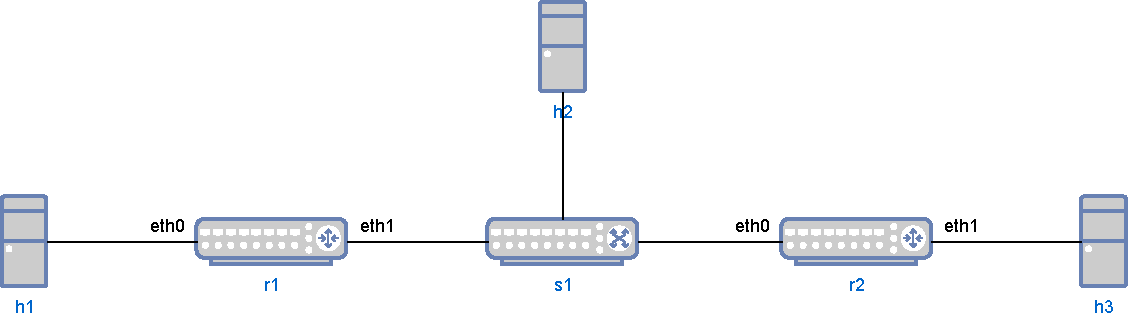
\includegraphics[width=\linewidth]{graphics/Lab4-mininet1.pdf}	
	\caption{Network configuration}
	\label{fig:lab4-mininet1}
\end{figure}

\begin{table}[h!t]
	\centering
	\begin{tabular}{| c | c | c |}	
		\hline
		\textbf{Host} & \textbf{eth0} & \textbf{eth1} \\ \hline
		h1 & \ipaddr{fc00:0:0:1::1/64} & N/A \\
		h2 & \ipaddr{fc00:0:0:2::2/64} & N/A \\
		h3 & \ipaddr{fc00:0:0:3::3/64} & N/A \\ \hline
		r1 & \ipaddr{fc00:0:0:1::10/64} & \ipaddr{fc00:0:0:2::10/64} \\
		r2 & \ipaddr{fc00:0:0:2::11/64} & \ipaddr{fc00:0:0:3::10/64} \\ \hline
	\end{tabular}
	\caption{\ac{ip} addresses}
	\label{tab:lab4-mininet1}
\end{table}

In this lab, we will start with the topology shown in figure \ref{fig:lab4-mininet1}.
By default, when an \emph{ipmininet router} is instantiated, it starts up an \acs{ospf} daemon so that all routes in your topology are properly set automatically. Also, each \emph{host} is configured with a default route to one of the routers in its subnet(s).

In this exercise, we want to have a look at the routing tables without \acs{ospf} automatically updating them. You can do this by specifying some parameters in you script:

\begin{itemize}
	\item First of all, make sure you add \incommand{from ipmininet.router.config import RouterConfig, STATIC, StaticRoute} to your script.
	\item Secondly, every time you create a router, add an extra parameter \incommand{config=RouterConfig} to the router definition.
\end{itemize}

This will make sure the routers do not start up an \acs{ospf} daemon automatically.

\begin{exercise}{Configuring static routes}
	\begin{enumerate}
		\item Write a python script to implement the above topology \textbf{and make sure the OSPF daemons are not started on the routers!} Save the script to \file{py}.
		\item Start the mininet script, and issue a \incommand{pingall} command. Save the output of the \incommand{pingall} to \file{pingall.txt}
		\item On every host and router, inspect the \textbf{\acs{ipv6}} routing table using either the \incommand{ip -6 route show} command. Save the routing tables to \file{routes.before.txt} (and indicate which routing table belongs to which host).
	\end{enumerate}

	\question{Using the output of the routing tables and of the \incommand{pingall} command, explain which pings succeed and which pings fail and why.}{1}
	\question{Which hosts or routers need to be configured with one or more extra routes? Indicate \textbf{which routes} need to be added.}{1}
	\question{Are there hosts or routers that do not require extra routes? Why (not)?}{1}

	Add the required routes to the hosts and/or routers using the \incommand{ip route -6 add} command (look up the exact syntax required). When you are done, verify with \incommand{pingall} that all hosts can now reach each other. Save the output of the routing tables again to \file[4]{routes.after.txt}.

	\question{Include the output of all routing tables:}{1}

	\question{From h1, perform a \incommand{traceroute} to h3,  using the \incommand{-q 1 -N 1 -z 100} options, and then a second time using the additional \incommand{-I} option. While doing the traceroutes, run a wireshark capture on eth0 of r1 and save it to \linktrace[5]{pcapng}. Using the trace file, explain how traceroute works in both cases (with and without the \incommand{-I} option).}{2}
\end{exercise}

\begin{exercise}{Routing loops}
	\begin{figure}[h!t]
		\centering
		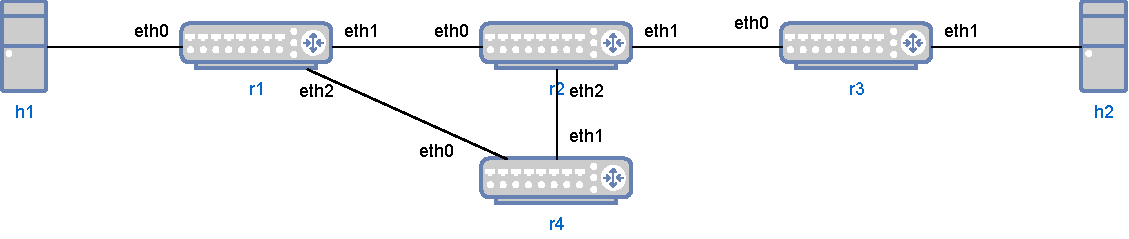
\includegraphics[width=\linewidth]{graphics/Lab4-mininet2.pdf}	
		\caption{Network configuration for routing loops}
		\label{fig:lab4-mininet2}
	\end{figure}
	
	\begin{table}[h!t]
		\centering
		\begin{tabular}{| c | c | c | c |}	
			\hline
			\textbf{Host} & \textbf{eth0} & \textbf{eth1} & \textbf{eth2} \\ \hline
			h1 & \ipaddr{fc00:0:0:1::1/64} & N/A & N/A \\
			h2 & \ipaddr{fc00:0:0:6::2/64} & N/A & N/A \\ \hline
			r1 & \ipaddr{fc00:0:0:1::11/64} & \ipaddr{fc00:0:0:2::11/64} & \ipaddr{fc00:0:0:5::11/64} \\
			r2 & \ipaddr{fc00:0:0:2::12/64} & \ipaddr{fc00:0:0:3::12/64} & \ipaddr{fc00:0:0:4::12/64} \\
			r3 & \ipaddr{fc00:0:0:3::13/64} & \ipaddr{fc00:0:0:6::13/64} & N/A \\
			r4 & \ipaddr{fc00:0:0:5::14/64} & \ipaddr{fc00:0:0:4::14/64} & N/A \\ \hline
		\end{tabular}
		\caption{\ac{ip} addresses for routing loops}
		\label{tab:lab4-mininet2}
	\end{table}

	Routing loops occur when a router that forwards a packet, receives the same packet later again, causing it to forward the same packet again (over the same path). This can happen again and again and is obviously a waste of resources. Moreover, the forwarded (looped) packet will never reach its intended destination. We will start from the topology shown in figure \ref{fig:lab4-mininet2}. As was the case in the previous exercise, write a python script that creates the following topology and \textbf{make sure no routing daemons are started by default!} Save it to \file{py}.

	\begin{enumerate}
		\item Start your python script and add routes so that:
			\begin{itemize}
				\item r1 will send traffic to the subnet of h2 to eth0 of r2.
				\item r2 will send traffic to the subnet of h2 to eth1 of r4.
				\item r4 will send traffic to the subnet of h2 to eth2 of r1.
				\item r2 and r4 have a route to h1 via r1.
			\end{itemize}
		\item Start a wireshark capture on eth0 of r2 and save it to \file{pcapng}.
		\item Start a ping command from h1 to h2. \emph{Limit the amount of pings to just 1!}
		\item After the ping, also send a \incommand{traceroute} from h1 to h2. Perform the traceroute commands with the \incommand{-q 1 -N 1 -z 100} options. Save the output to \file[3]{traceroute.txt}.
	\end{enumerate}

	\textbf{Use the data captured with Wireshark in \linktrace[1]{pcapng} to answer the questions. Support your answers with the saved Wireshark data.}

	\question{In the trace file, identify two consecutive looped ping packets. Are they identical? If not, what is different?}{1}
	\question{How many times does the looped ping packet appear in your trace file? Why doesn't it loop forever?}{1}
	\question{Include your traceroute output in the answer below. In that output, you should clearly see the routing loop. Using this output and the packets in the trace file, explain what happens.}{2}
\end{exercise}

\newpage
\section{\acl{bgp}}\label{sec:bgp}

In the previous exercises, you learned how to configure routing table entries manually. This was referred to as static routing. The topic of the next exercises is dynamic routing, where dynamic routing protocols (from now on, called routing protocols) set the routing tables automatically without human intervention. Routers and hosts that run a routing protocol, exchange routing protocol messages related to network paths and node conditions, and use these messages to compute paths between routers and hosts.

Most routing protocols implement a shortest-path algorithm, which, for a given set of routers, determines the shortest paths between the routers. Some routing protocols allow that each network interface be assigned a cost metric. In this case, routing protocols compute paths with least cost. Based on the method used to compute the shortest or least-cost paths, one distinguishes distance vector and link state routing protocols.

In a link-state algorithm, the network topology and all link costs are known, that is, available as input to the LS algorithm. In practice, this is accomplished by having each node broadcast link-state packets to all other nodes in the network, with each link-state packet containing the identities and costs of its attached links. In practice (for example, with the Internet's \acs{ospf} routing protocol), this is often accomplished by a link-state broadcast algorithm. The result of the nodes' broadcast is that all nodes have an identical and complete view of the network. Each node can then run the LS algorithm and compute the same set of least-cost paths as every other node.

Whereas the LS algorithm is an algorithm using global information, the distance-vector (DV) algorithm is iterative, asynchronous, and distributed. It is distributed in that each node receives some information from one or more of its directly attached neighbours, performs a calculation, and then distributes the results of its calculation back to its neighbours. It is iterative in that this process continues on until no more information is exchanged between neighbours. The algorithm is asynchronous in that it does not require all of the nodes to operate in lockstep with each other.


The notion of an autonomous system (AS) is central to the understanding of routing protocols on the Internet. An autonomous system is a group of \ac{ip} networks under the authority of a single administration, and the entire Internet is carved up into a large number of autonomous systems. A list of all AS's can be found on the \href{https://www.bgplookingglass.com/list-of-autonomous-system-numbers}{BGP Looking Glass} website. Examples of autonomous systems are \emph{Belnet}, \emph{Telenet}, \emph{Proximus}, etc. Each autonomous system is assigned a globally unique identifier, called the AS number. On the Internet, dynamic routing within an autonomous system and between autonomous systems is handled by different types of routing protocols. A routing protocol that is concerned with routing within an autonomous system is called an intradomain routing protocol or interior gateway protocol (IGP). A routing protocol that determines routes between autonomous systems is called an interdomain routing protocol or exterior gateway protocol (EGP).

We will start with interdomain routing by having a look at the \ac{bgp} protocol.

\begin{exercise}{\acs{bgp}}
	In this exercise, things are a bit different. You will find a file called \incommand{bgp.py} as an extra to this lab. This file contains the setup for the following exercise. This setup has also \emph{disabled} any standard \acs{ospf} daemons in mininet, but has added \acs{bgp} daemons instead that are responsible for exchanging \acs{bgp} routing information. Additionally, on \texttt{as1rb}, a wireshark trace is automatically started on all interfaces simultaneously when the script starts, so you will be capturing all traffic from the beginning. After the script is stopped, the trace file can be found in \path{/tmp/bgp_as1rb.pcapng}.

	\question{Study the \incommand{bgp.py} file and make a drawing of the topology it creates. Also include a table with the interface names and \acs{ip} addresses that are being used. Finally, since we are going to use \acs{bgp}, on your drawing, indicate which router belongs to which AS.}{1}

	\begin{enumerate}
		\item Start the \incommand{bgp.py} topology in mininet.
		\item Wait a few seconds for the topology to settle. When \incommand{pingall} reports a 100\% success rate, you can continue with the next step.
		\item From h1b, issue a traceroute to h2b. Save the output to \file[3]{traceroute.txt}.
		\item Bring the \incommand{eth3} interface of as1rc down using \incommand{ifconfig}.
		\item Perform a traceroute again from h1b to h2b and add the output to \file[3]{traceroute.txt}.
		\item Bring the \incommand{eth3} interface of \incommand{as1rc} back up. \textbf{Do not forget to configure the IP address of that interface again, as it will have been removed from that interface!}
		\item Again, perform a traceroute from h1b to h2b and add the output to \file[3]{traceroute.txt}.
		\item Stop the script. Rename the wireshark trace found in \path{/tmp} to \file[2]{as1rb.pcapng}.
	\end{enumerate}

	\textbf{Use the data captured with Wireshark in \linktrace[2]{as1rb.pcapng} to answer the questions. Support your answers with the saved Wireshark data.}

	\question{Open the wireshark trace file and take a look at the \acs{bgp} packets that were captured. Which types of \acs{bgp} messages did you capture and what is their purpose? Refer to  packet numbers in the trace for examples of those messages.}{2}
	\question{How did the route change when you brougth the interface down? How did it change when you brought it back up again?}{1}
	\question{Why did \acs{bgp} decide upon the original route (before the interface was brought down)?}{1}
	\question{Explain \emph{in detail} using the \acs{bgp} packets in your wireshark trace how \texttt{as1rb} knows how to change the routes so h1b and h2b can continue to communicate (when the link is taken down and again when it is brought back up). Explain the different fields in the \acs{bgp} messages that are used to distribute the necessary information and explain their meaning.}{5}
\end{exercise}

\newpage
\section{\acl{ospf}}\label{sec:ospf}

In this exercise, you explore the \acf{ospf} routing protocol. \acs{ospf} is a link state routing protocol, where each router sends information on the cost metric of its network interfaces to all other routers in the network. The information about the interfaces is sent in messages that are called link state advertisements (LSAs). LSAs are disseminated using flooding, that is, a router sends its LSAs to all its neighbours, which, in turn, forward the LSAs to their neighbours, and so on. However, each LSA is forwarded only once. Each router maintains a link state database of all received LSAs, which provides the router with complete information about the topology of the network. Routers use their link state databases to run a shortest path algorithm that computes the shortest paths in the network.

\ac{ospf} is the most important link state routing protocol on the Internet. The functionality of \ac{ospf} is rich, and the lab exercises highlight only a small portion of the \ac{ospf} protocol. In this exercise, we use \ac{ospf} version 3 (\ac{ospf}v3).

\begin{exercise}{\acs{ospf}}
	You once again can find a pre-existing topology for the \acs{ospf} setup in \incommand{ospf.py}. This topology is basically a subset of the topology in the previous exercise. AS number 1 is extracted from that topology, and all the routers in that topology are now configured to run \acs{ospf}. Similar to the previous exercise, when you start up the script, a wireshark capture logging all traffic on all interfaces of as1ra is automatically started. It is saved to \path{/tmp/ospf_as1ra.pcapng}.
	
	\question{Study the \incommand{ospf.py} file and make a drawing of the topology it creates. Also include a table with the interface names and \acs{ip} addresses that are being used. Finally, since we are going to use \acs{ospf}, on your drawing, indicate which weights (called \texttt{igp\_metric} in the script) are configured on each link.}{1}

	\begin{enumerate}
		\item Start the \incommand{ospf.py} script.
		\item Because of the topology and configuration choices in the script, it takes a while before all routes are ready. After about 30 seconds, this should be the case. Check that a \incommand{pingall} command reports a 100\% success rate before continuing.
		\item On h1a, start three pings (one to each of h1b, h1c and h1d). Don't set any parameters, but just let the pings continue to run. Save the output of the ping commands to \file{ping-h1X.txt}, where X is b, c or d, respectively.
		\item From h1a, issue a \incommand{traceroute} to all other hosts (just the hosts, not the routers). Do the same from host h1d. Save the output of both traceroutes to \file{traceroute.1.txt}.
		\item Bring down the link between as1ra and as1rc. \textbf{Do this on as1rc as it will otherwise interfere with the wireshark capture that is running on as1ra!}
		\item Do the same traceroutes as above, and save the output to \file{traceroute.2.txt}.
		\item Now, also bring down the link between as1ra and as1rb and between as1rb and as1rd.
		\item Again perform the same traceroutes, and save the output to \file{traceroute.3.txt}.
		\item Bring all the interfaces back up one by one \textbf{and don't forget to set the IP address on them again!} After bringing the interfaces up, monitor the ping commands until you notice the routes have changed and settled.
		\item Finally, verify that, now all links are back up, your traceroutes yield the same results as in the beginning of the exercise.
		\item Stop the pings and the mininet script. Rename the wireshark capture to \file{pcapng}.
	\end{enumerate}

	\textbf{Use the data captured with Wireshark in \linktrace[1]{pcapng} to answer the questions. Support your answers with the saved Wireshark data.}

	\question{Explain the routes you obtained when you did the first set of \incommand{traceroutes}. Why are the routes what they are?}{1}
	\question{After you brought down the first interface, which routes changed and what are the new routes? Focus only on the routes starting at h1a and h1d, and refer to your traceroute output.}{1}
	\question{When you brought down the first interface, you should have seen \acs{ospf} packets in your trace file. Which packets are those and what is their purpose?}{1}
	\question{Explain \emph{in detail} using the \acs{ospf} packets in your wireshark trace how the routers know how to change the routes so all hosts can continue to communicate. Explain the different fields in the \acs{ospf} packets that are used to distribute the necessary information and explain their meaning.}{3}
	\question{When you brougth the interfaces back up one by one, did the routes change again? Why? How do the routers decide to change their routes?}{2}
	\question{Did it take longer or shorter for the routes to change when the interfaces were brought back up than when they were brought down? Why?}{1}
\end{exercise}

\newpage
\section{\ac{bgp} and \acs{ospf} Combined}\label{sec:bgp}

\begin{exercise}{Bringing everything together}
	Now that you have configured \acs{bgp} for exchanging inter-AS routing information, and \acs{ospf} for intra-AS routing, it is time to bring everything together. Starting from the \incommand{bgp.py} and \incommand{ospf.py} scripts, you need to create a new script called \incommand{bgp\_ospf.py}, that satisfies the following requirements:

	\begin{enumerate}
		\item The topology in the script is the same topology as in the \incommand{bgp.py} script, except that, in every AS, the direct link between \incommand{asXra} and \incommand{asXrc}, and the direct link between \incommand{asXrb} and \incommand{asXrd} are \textbf{removed}.
		\item The \acs{bgp} configuration remains the same as in the \acs{bgp} exercise.
		\item Within each AS, \acs{ospf} is used to exchange routing information.
		\item There is \textbf{no \acs{ospf} traffic} between the different AS.
	\end{enumerate}

	\begin{remark}
		Consult \href{https://ipmininet.readthedocs.io/en/latest/daemons.html#ospf6}{the ipmininet documentation} on how to disable \acs{ospf} on an interface.
	\end{remark}

	Once you have created the specified topology, perform the following steps:

	\begin{enumerate}
		\item Start the \incommand{bgp\_ospf.py script}.
		\item Wait for the topology to settle. If everything is configured correctly, a \incommand{pingall} command should report a 100\% success rate.
		\item Create a scenario involving \emph{at least} traceroute commands to be able to identify the route a packet takes from a certain host to another host. The scenario should cover the following:
		\begin{itemize}
			\item You should have a ping/ssh/iperf/... connection between two hosts in a different AS. (When using iperf, you should make sure any trace files you make do  not get too big by limiting the iperf bandwidth and/or the link bandwidth in your topology.)
			\item Start up wireshark traces on a relevant interface that will contain \acs{bgp} traffic, as wel as on an interface that will contain \acs{ospf} traffic. \emph{Do not forget to include these traces as attachment to this lab report!}.
			\item At every step of the scenario, check the actual route between the two hosts with \incommand{traceroute}.
			\item You should break the link on the initial path between the two AS systems and check how the routes are changed.
			\item You should also break \emph{at least one link} within the same AS that is on the path between both hosts and check how the routes are changed.
			\item You should also re-enable the links you brought down and check how the routes are changed.
			\item Whenever bringing down links, verify that at all times a valid path exists between the two hosts you are using in your scenario.
		\end{itemize}

		\question{Make a drawing of your final topology. Include any details such as AS numbers, link weights, etc. Include all relevant output as extra files and mention them in your answer (traceroute output, ping output, iperf output, ...). Also, the wireshark captures should be included. Clearly mention which capture was made on which interface. Explain \emph{in detail} the different steps in your scenario, and for every step, explain how and when the topology changes. Things to take into consideration:
		\begin{itemize}
			\item Does the topology change immediately, or does it take a while? Why?
			\item Is there any packet loss? Why?
			\item How do the routers know how to change the topology?
			\item When the topology is changed (e.g. a link is brought up or down): how far does this information travel (i.e. which routers are informed)? Why?
		\end{itemize}
		The above questions apply both when taking down the interfaces, as well as when you bring them back up!}{15}
	\end{enumerate}

\end{exercise}
